\chapter{Networking Addendum}

\section{Seam Carving}
\label{app:seamCarving}

\indent \indent
In the original seam carving paper, Avidan and Shamir proposed multiple energy functions to attempt to quantify the importance of a pixel in order to remove ``those which won't be noticed'' ~\cite{SeamCarving}.
\smallskip \\ \indent
To begin with, Equation \ref{eq:energy1} is proposed. It is then evolved into Equation \ref{eq:energy2} to achieve better results by using a histogram to group pixels.
\begin{equation}
    \label{eq:energy1}
    e(\vec{I}) = \left| \frac{\partial}{\partial x} \vec{I} \right| + \left| \frac{\partial}{\partial y} \vec{I} \right|
\end{equation}
\begin{equation}
    \label{eq:energy2}
    e_{\textit{HoG}}(\vec{I}) = \frac{\left| \frac{\partial}{\partial x} \vec{I} \right| + \left| \frac{\partial}{\partial y} \vec{I} \right|}{\max{(\textit{HoG}(\vec{I}(x,y)))}}
\end{equation}
where $\textit{HoG}(\vec{I}(x,y))$ is a histogram of oriented gradients at every pixel. The paper recommended an eight-bin histogram over an eleven-pixel square window around each pixel. Figure \ref{fig:scEnergy} depicts the application of an energy function to an example image.
\smallskip \\ \indent
Once the energy of each pixel has been calculated, the seams of the image need to be generated. This allows the optimal seam to be determined and deleted from the image. To do this, the cost of a seam can be quantified by Equation \ref{eq:seamCost}. The dynamic programming algorithm originally proposed is defined by Equation \ref{eq:dpSeamCarving} - for vertical seams, the equation for horizontal seams is similar.
\begin{equation}
    \label{eq:seamCost}
    E(\vec{s}) = E(\vec{I_s}) = \sum^n_{i=1} = e(\vec{I}(s_i))
\end{equation}
\begin{equation}
    \label{eq:dpSeamCarving}
    M(i, j) = e(i,j) + \min{(M(i-1, j-1), M(i-1, j), M(i-1, j+1))}
\end{equation}
\bigskip \\ \indent
The figure below depicts each stage of the seam carving algorithm. Images are taken from \cite{wikiSeamCarving}.


\begin{figure}[htp]
    \begin{subfloatrow}
        \floatbox[{\capbeside\thisfloatsetup{capbesideposition={right,center},capbesidewidth=3.7cm}}]{figure}[\FBwidth]
        {\caption{Original image.}}
        {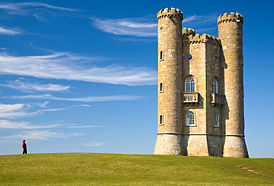
\includegraphics[scale=.7]{figures/seamCarving1.png}}
    \end{subfloatrow}
    \begin{subfloatrow}
        \floatbox[{\capbeside\thisfloatsetup{capbesideposition={right,center},capbesidewidth=5cm}}]{figure}[\FBwidth]
        {\caption{The energy of each pixel.}\label{fig:scEnergy}}
        {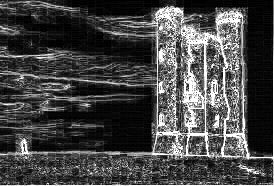
\includegraphics[scale=.7]{figures/seamCarving2.png}}
    \end{subfloatrow}
    \begin{subfloatrow}
        \floatbox[{\capbeside\thisfloatsetup{capbesideposition={right,center},capbesidewidth=5cm}}]{figure}[\FBwidth]
        {\caption{Potential seams to delete.}\label{fig:scSeams}}
        {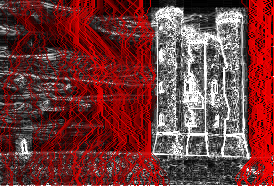
\includegraphics[scale=.7]{figures/seamCarving3.png}}
    \end{subfloatrow}
    \begin{subfloatrow}
        \floatbox[{\capbeside\thisfloatsetup{capbesideposition={right,center},capbesidewidth=11cm}}]{figure}[\FBwidth]
        {\caption{Low energy seams removed.}\label{fig:scRemoved}}
        {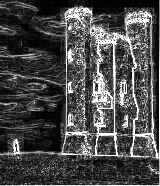
\includegraphics[scale=.7]{figures/seamCarving4.png}}
    \end{subfloatrow}
    \begin{subfloatrow}
        \floatbox[{\capbeside\thisfloatsetup{capbesideposition={right,center},capbesidewidth=9.5cm}}]{figure}[\FBwidth]
        {\caption{Resulting image.}}
        {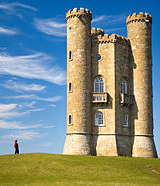
\includegraphics[scale=.7]{figures/seamCarving5.png}}
    \end{subfloatrow}
    \caption[Seam Carving Stages]{Each stage of the seam carving algorithm.}
\end{figure}



\pagebreak



\section{Sliding Window}
\label{app:slidingWindow}
\indent \indent
A sliding window protocol is a common approach to achieving reliable, in-order delivery in packet-based data transmission protocols. Their main advantage over other techniques is that they can improve transmission efficiency in a channel with high latency. The first stage of the algorithm requires a buffer to be created storing all packets, and each packet to be assigned an identifier. Then, a window size, $n$, is defined. This value determines the number of packets that will be in flight between the sender and receiver simultaneously. Initially, the first $n$ packets will be sent in a single batch.
\smallskip \\ \indent
Whenever a packet arrives at its destination, an acknowledgement containing the identifier of the packet is returned to the sender. This causes the sender to increment the sliding window, and the next packet in the buffer transmitted. If the acknowledgement is not received - possibly because the original packet was lost in transmission, or because the acknowledgement was - the sender will retransmit a packet after a timeout has expired. Two techniques for ensuring reliable transmission are included below.
\subsection{Go-Back-N ARQ}
\indent \indent
The Go-Back-N Automatic Repeat Request protocol recovers from packet loss or corruption by resending the target packet as well as all subsequent packets in the window. The N in the name of this protocol refers to the size of the window. This method minimises the complexity of the network, so is often preferred.
\subsection{Selective Repeat ARQ}
\indent \indent
The Selective Repeat Automatic Repeat Request protocol recovers from packet loss or corruption by resending the target packet alone. This method is more appropriate if lots of loss is expected because the traffic on the network is minimised. 
\smallskip \\ \indent
Figure \ref{fig:slidingWindow} summarises the sliding window approach to data transmission succinctly.
\begin{figure}[htp]
    \begin{subfigure}[b]{0.45\textwidth}
        \centering
        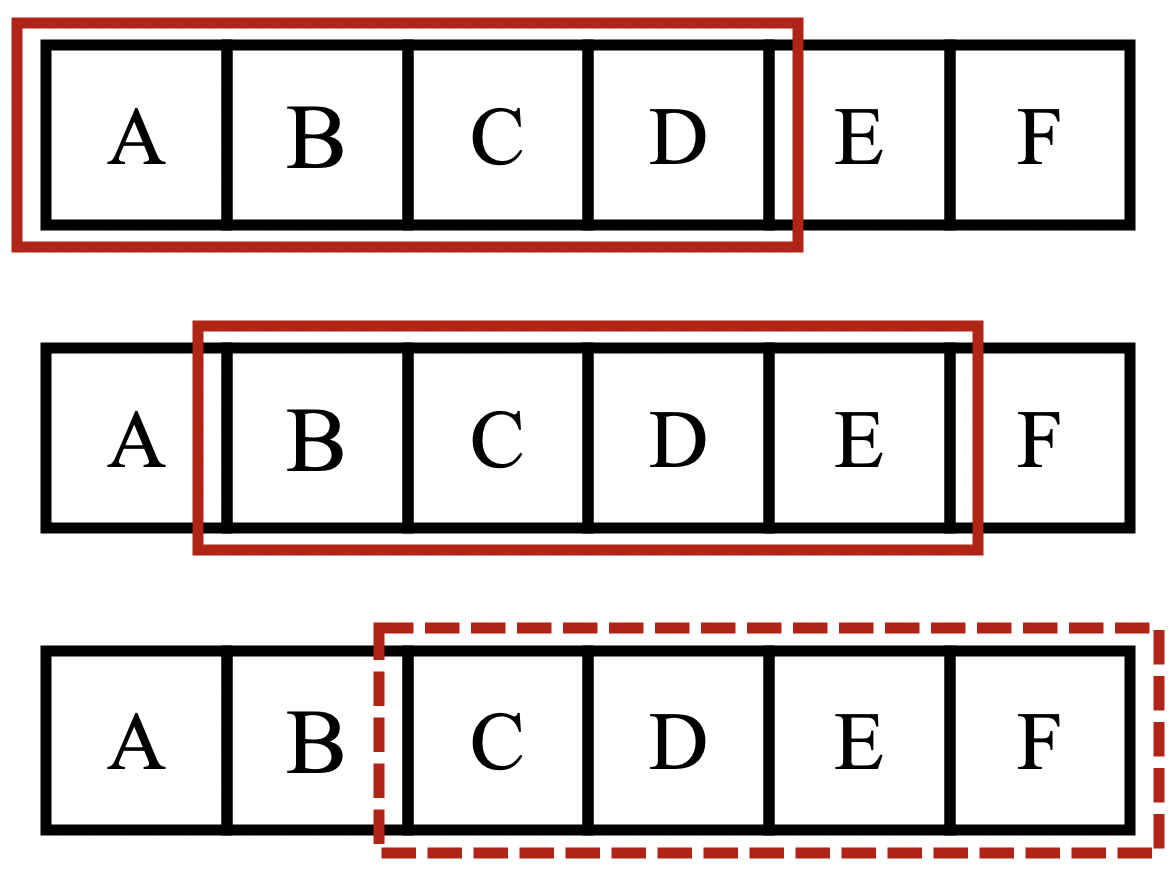
\includegraphics[scale=0.25]{figures/slidingWindow1}
        \caption{The sliding window (red) moves across the packets as each one is sent. Initially the first four packets are sent (top). When packet A is acknowledged, the window slides along one, and E is sent (middle). After the acknowledgement for B is received the window will slide along for F to be sent (bottom).}
    \end{subfigure}\hfill%
    \begin{subfigure}[b]{0.45\textwidth}
        \centering
        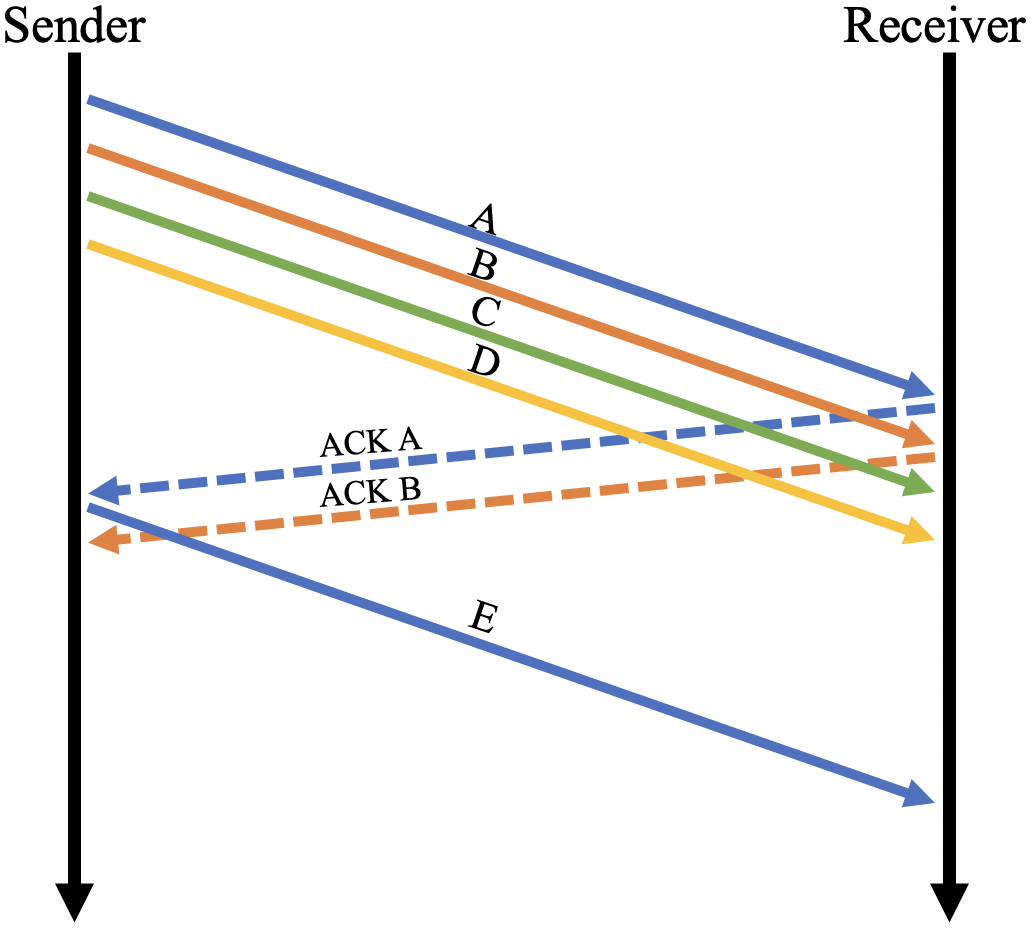
\includegraphics[scale=0.3]{figures/slidingWindow2}
        \caption{The packets currently in the window are sent at the same time, without waiting for any acknowledges. Once an acknowledgment has been received, the next packet in the queue can be sent.}
    \end{subfigure}%
    \caption[The Sliding Window Protocol]{A high-level view of TCP's sliding window protocol.}
    \label{fig:slidingWindow}
\end{figure}
